\section{Background}
\label{sec:background}

\subsection{The field}

A finite field with $p^k$ elements can be built from polynomials of degree less than $k$
whose coefficients are integers modulo the prime $p$~\cite{lidl1997finite}. Two elements are
added coefficient by coefficient. They are multiplied as polynomials and the product is then
reduced modulo a fixed irreducible polynomial of degree $k$. The assignment uses $p = 11$ and
$k = 3$, so there are $11^3 = 1331$ elements. The library does not hard-code the modulus. It
enumerates monic cubics in a fixed order and takes the first irreducible one, which is
$x^3 + x + 4$. Any replacement has to keep that choice, because a different modulus gives a
different multiplication table.

\subsection{The dependency chain}

Fig.~\ref{fig:dependencies} shows the repositories involved. All of them are header-only
C++20 libraries that CMake fetches at pinned commits. The assignment program uses two of them
directly: \code{algebra-matrices} for the matrix product, and \code{algebra-finite-fields}
for the element type. The finite field class in turn stores a polynomial from
\code{algebra-polynomials}, whose coefficients are residues from \code{algebra-rings}, which
are built on the cyclic groups of \code{algebra-groups}.

\begin{figure}[t]
  \centering
  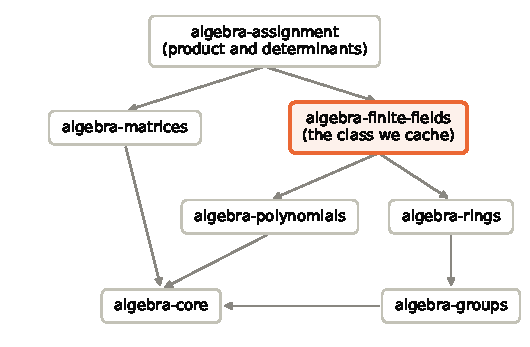
\includegraphics[width=\columnwidth]{figures/dependencies.pdf}
  \caption{The dependency chain. An arrow points from a repository to one it depends on.
  Everything below \code{algebra-finite-fields} is reached only through the finite field
  class.}
  \label{fig:dependencies}
\end{figure}

The layers are written for clarity, not speed, and the costs multiply. One field
multiplication multiplies two polynomials, which is up to nine coefficient products. Each
coefficient product is carried out by repeated addition. The product polynomial is then
divided by the modulus to get the remainder. Every intermediate polynomial is a
\code{std::vector} allocated on the heap.

\subsection{The workload}

The matrix product performs $N^3$ field multiplications and $N^3$ additions. Each
determinant is a Gaussian elimination with about $N^3/3$ multiplications, negations and
additions. In total the program asks for about $5N^3$ field operations, which is
$3.2 \times 10^{11}$ for $N = 4000$. The operands of all of them come from only 1331
values, so a binary operation has only $1331^2 = 1\,771\,561$ distinct inputs. Each one is
therefore recomputed tens of thousands of times, which is the situation caching is for.
